
% Distributed under the MIT License.
% (See accompanying file LICENSE.txt)
% (C) Copyright NoWork team

\documentclass[12pt,a4paper]{article}

\usepackage[utf8]{inputenc}
\usepackage[american]{babel}
\usepackage[T1]{fontenc}
\usepackage{listings}
\usepackage{graphicx}
\usepackage{dirtree}

\lstset{language=Caml}

\title{NoWork\\
Developer manual}
\author{NoWork development team\\[2em]}
\date\today

\begin{document}
\maketitle

\section{Introduction}

This document presents to developers NoWork, a nominal rewriting workbench. Anyone interested by the mechanisms of NoWork or rewriting system in general might find interests in this document. It is also essential if you want to modify this project. We expect that you first read the user manual and played a bit with the interpreter. If you intend to modify this project and provide a pull-request, you can read the coding style document.
\newline

The section \ref{install} prepares you to hack on NoWork by installing everything needed, we next give an overview of the global architecture in section \ref{architecture}. The modules presented are further described in the following sections, the top-level is presented in section \ref{top-level}. The data structures encoding the language are presented in section \ref{data-system} and we highlight the different representation occurring during the system processing. The section \ref{data-term} shows different term structure and more particularly, explains how the hash-consing is working and why it is important in this project. The typing phase is described in section \ref{typechecking} and is followed by the algorithms section. The algorithm selecting a rule via its pattern is presented in the section \ref{pattern-matching}, the matching rules are then applied to a term with a specific strategy, the section \ref{rewriting} is dedicated to the rewriting algorithm. This document concludes with a rational in section \ref{rational} discussing the different high-level choices and why we make these choices.

\section{Installing and hack on NoWork}
\label{install}
%% Matthieu
How to install and begin to develop with NoWork.

\section{Architecture}
\label{architecture}
%% Mathieu

Here comes a simplified description of the directory layout :
\bigskip

\dirtree{%
.1 /.
.2 doc.
.2 data.
.3 error.
.3 test.
.4 run-pass.
.4 run-fail.
.2 src.
.3 algorithms.
.3 auto\_gen.
.3 generator.
.3 interactive.
.3 parser.
.3 system.
}
\bigskip

And now a more precise description of these directories :

\begin{itemize}

\item \emph{doc} : obviously contains documentation files (user manual, developper manual, coding style, ...)
\item \emph{data/error} : custom exceptions declaration in \emph{*.conf} files (need to be declared here to be used in tests)
\item \emph{data/test} : functional tests framework, test files are added in either \emph{run-fail} or \emph{run-pass}, and test expectations in \emph{test.nw}
\item \emph{src/algorithms} : general algorithms that don't rely on one particular system such as matching and rewriting
\item \emph{src/generator} : generated errors system
\item \emph{src/interactive} : top-level system
\item \emph{src/system} : contains the different AST representations, type checking modules (\emph{type\_checking} and \emph{term\_checker}), and symbol tables

\end{itemize}

\section{Top-level}
\label{top-level}
%% Vincent

The top-level interface is classically designed. First, we parse the
given phrase. Then, we evaluate it, eventually modifying the current
system. Outputting the result if any and finally give back the hand to
the user. 

\bigskip
To add new directives, the process is simple. First, you will need to
add a new directive in the concerned table in the lexer :
\verb?src/parser/lexer.mll?. Then, add the corresponding grammar rule
in the parser : \verb?src/parser/parser.mly?\footnote{Please consult
  the official ocamllex and ocamlyacc documentation if difficulties
  are encountered hacking into those files}. You will also need to add
a new branch in the \verb?interactive_ast? OCaml sum type in
\verb?src/parser/parsing_ast.ml? (and its \verb?.mli? interface). Now,
we need to evaluate this directive. To achieve that, we have to add a
match-case in the \verb?eval_interactive_cmd? located
\verb?src/interactive/eval.ml?. It's recommanded to add a quick how-to
description of the newly implemented command in the usage at the
beginning of the last file. 

The current implementation uses prettifying functions to gracefully
display the resulting expressions. It relies on the \verb?Format?
standard OCaml library. The file containing these functions is :
\verb?src/system/pretty.ml?

\section{Parsing and data representation}
\label{data}

\subsection{System representation}
\label{data-system}
%% Rémy
Which transformation of the representation of the system occurred and
why?

\subsection{Term representation}
\label{data-term}
%% Pierrick Matthieu
During the process between the parsing and the rewriting of a term, the
structure reprensenting the term is transformed step by step.

\subsubsection{From parsing to semantic-checking}
Parsed terms are transformed in the following \verb?term_ast? :
\begin{lstlisting}
  type info = Lexing.position

  type ident = string

  type term_desc =
  | Const
  | Term of term_ast list
  | Var

  and term_ast =
  {
    name : string;
    info : info;
    desc : term_desc;
  }
\end{lstlisting}

This AST is used only to keep position (in the original file) and structure
informations.
But it is made using only grammatical informations, so it can be
semantically incoherent. That is why it will be transformed during the
type-checking.

\subsubsection{From semantic-checking to type-checking}
The second transformation take a \verb?term_ast? and use semantic informations
contained in the rewriting system to check the semantic of the AST (term
arity and well definition of each symbol)  then
construct an AST with that additional informations (differentiation between
bounded atoms and atom's binders). Now, the term is ready to be type-checked.
\\
N.B. : This AST is called \verb?term_ast_with_binders? (because of his
author's lack of inspiration) in the \verb?term_ast_typed.ml?.
It constructed by \verb?construc_ast_checked? in \verb?term_checker.ml?

\subsubsection{From type-checking to hash-consing}
At the end, the type-checking, processed on the precedent AST, gives a
typed AST keeping only structure and type informations of the original AST.
It is made by \verb?check_type_of_term?.
\\
A term passing all of the steps is considered as wel formed and typed, then
the user can manipulate and particulary rewrite it. In order to have an
efficient rewriting the AST must be transformed a last time.

\subsubsection{Hash-consing}
\label{data-term-hash-consing}
%% Pierrick
The hashconsing allows to express the structural equivalence (without
congruence) by only allocating once two terms that are identical. To do so, we
have to completely drop the names of binders and binded variables. The result is
a term that looks a lot like the typed terms, with some subtlety with the
binders and the binded variables.

The type is the following:
%% Lstlisting one
\begin{verbatim}
type 'a hashed = private { id: id; hash : int; value : 'a }

type 'a hlist = 'a hashed list

type hterm_raw = private
  | HConst of ident
  | HTerm of ident * hterm_raw hlist
  | HBinder of id hlist (* refers to the id of the head of an hashconsed
                           list. *)
  | HVar of int
  | HFreeVar of ident
\end{verbatim}

The most difficult part lies in the HBinder and HVar parts. To explain how it is
constructed, the best idea is to explain the algorithm. 

We cross our typed term from left to right, than at the end of the traversal, we
go back to effectively create our hashconsed subterms. The second part is
mandatory: when we create the subterms of a HTerm, the lsit has to be hashconsed
and we have to begin by the tail. Each cell of this hashconsed list is a record
containing a value and an id, which is the id of the actual hashconsed list
where this cell is the head of the list.

Now for the first part, it is moslty to capture the binders. And then while we
go from right to left, we capture the id of its binded variables that are in
hashconsed lists. This way, a binder is represented by an id list, which is
morally its binded variables. We just need to hashcons this id list and the
Binder can be hashconsed.

However, there is still one problem with this method, and this is solved by the
\texttt{HVar of int}. This is basically a de Bruijn index, which is mandatory
unfortunately. For example, imagine the following term 
\texttt{Lambda(x, Lambda(y, App(App(Var(y), Var(y)), App(Var(x), Var(y)))))}.
Without using de Bruijn, by using for example juste HVar (that would be
hashconsed once), the following pattern would match: 
\texttt{Lambda(?x, Lambda(?y, App(?T, ?T)))} because this would extract the vars
out of their context and they would became identical. Using the de Bruijn
indices solves this issue.

The hashing functions computes a hash value for each term and list. For list, it
computes from the head and tail. If its an empty list its value is zero, else it
is $head + 17 \times tail$ where $head$ and $tail$ are values given in
argument of the \texttt{hash\_value\_hlist} function. An extract from the code:
\begin{verbatim}
  let rec hash_hlist = function
    | [] -> 0
    | v :: [] -> hash_term v.value
    | v1 :: v2 :: _ -> hash_value_hlist (hash_term v1.value) v2.hash
\end{verbatim}
If you want to modify the hashing function, please change
\texttt{hash\_value\_hlist}, since it is used multiple times.

Finally, you can notice that a hterm is a record with the hashconsed term and a
name field. This is simply a tree mapping the names that were lost during the
hashconsing. This allows to recreate the typed term corresponding to the
hashconsed term.


\section{Type-checking}
\label{typechecking}
%% Ma(t.)hieu

\section{Algorithms}
\label{algorithms}

\subsection{Pattern-matching}
\label{pattern-matching}

The pattern matching algorithm returns a set of couple of placeholders and sub-terms regarding a pattern and a term. It is implemented in the files \texttt{src/algorithms/matching.\{ml,mli\}} and is well-commented. Consider the following extract of the Peano rewriting system:
\begin{lstlisting}
rule [add-l] :
  Add(Successor(?u), ?v) => Successor(Add(?u, ?v))

rule [add-r] :
  Add(?u, Successor(?v)) => Successor(Add(?u, ?v))

rule [div-same] :
  Div(?u, ?u) => Successor(Zero)
\end{lstlisting}

We simulate the pattern matching algorithm with the pattern of the rule \texttt{add-l} and the term \texttt{Add(Successor(Zero), Zero)} in figure \ref{peano-example}.

\begin{figure}
  \centering
  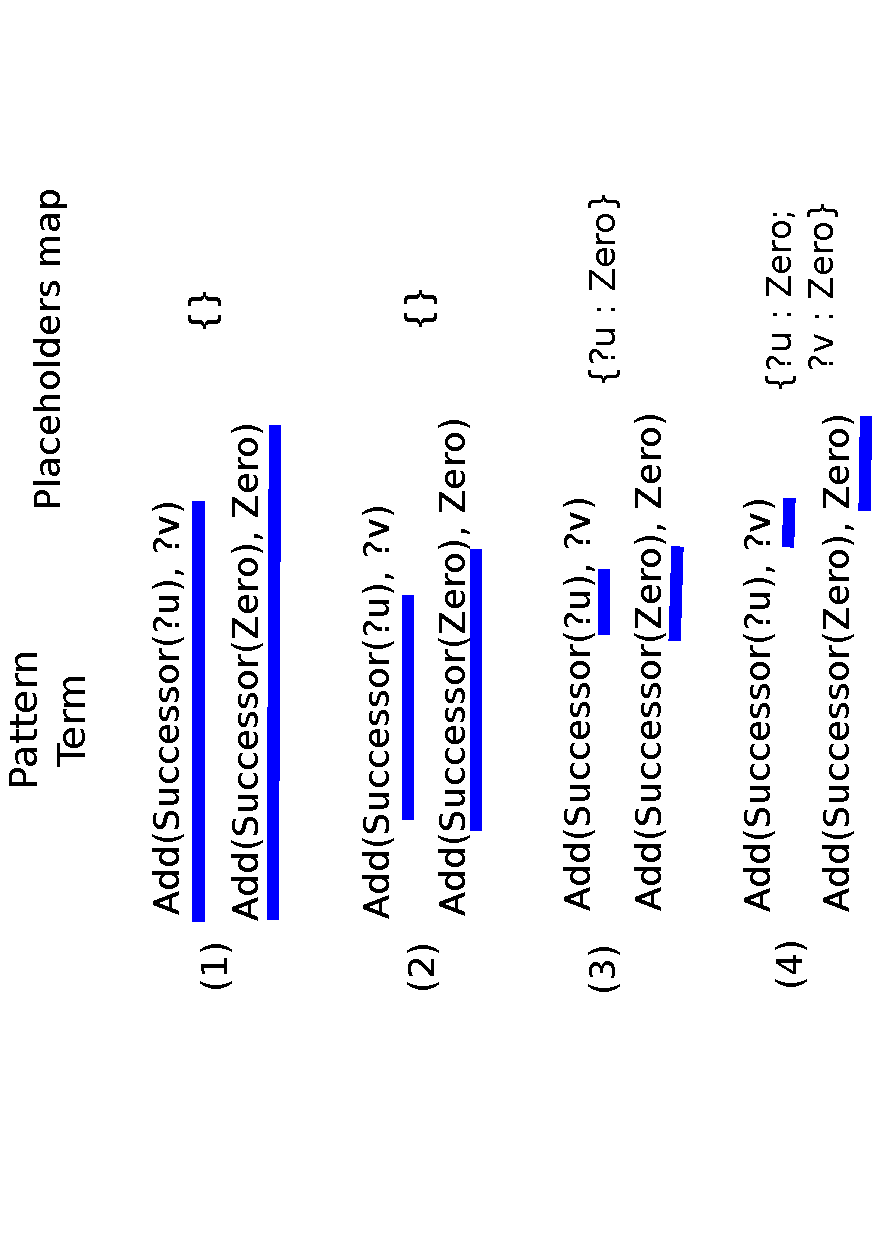
\includegraphics[scale=0.6, angle=270]{example-peano.pdf}
  \caption{Pattern matching on Peano term}
  \label{peano-example}
\end{figure}
g
The algorithm returns a type \texttt{map option}, if the term doesn't match the pattern, it returns \texttt{None}, otherwise it returns the bindings between the placeholders and sub-terms.
\newline

The algorithm is rather simple as it just travels at the same time the AST of the pattern and term. A problem appears in presence of non-linear pattern such as in the rule \texttt{div-same} because there are two identical placeholders. Comparing two terms modulo alpha-conversion have a bad complexity (it depends on the term length and on the number of binders). For this purpose, we firstly hash-consed our term as explained in section \ref{data-term-hash-consing} and we use it whenever we have to compare two sub-terms sharing a same placeholder. This have a constant complexity. We still need to go through the initial term since the hash-consed representation erased any notion of name and is useless to compare constant name and operators with patterns.

\subsection{Rewriting}
\label{rewriting}
%% Roven
The module rewriting contains all the algorithms needed to rewrite a term. There
are essentially two main operations, the basic rule rewriting and all the base
strategies functions. \\

The rule rewriting  function is rather simple, it will just call the matching module.
On success, it will call a function given in parameter with the resulting 
placeholders. On failure it wiil call another function. This architecture was coined
by a team member before the introduction of strategies, now this function is
called only in the rule base strategy and the success function is simply the 
substition and the failure function is simply returning the empty set.\\

Since the core of rewriting are the strategies, there architecture will be detailled
in the following subsection.

\subsection{Strategies}
The strategies are a rather independent addition to the whole program. Their AST is 
defined in the Strategy\_ast module, filled in the parser and the only module 
depending on them is Eval. 

\subsubsection*{AST}
The body of a strategy can be thought as just one big expression combining strategy
calls and operators. Therefore only one type was necessary to describe the AST, 
however, because of the stable nature the base strategies, all of them are 
hardcoded in the AST. For instance \verb|test(id())| will be directly translated into
\verb|STest(SId())|. This simplifies the base strategies checks because it is the 
OCaml compiler that does all the work.

\subsubsection*{Parsing}
The syntax was designed to blend easily with the rest the rewriting system. 
Strategies are therefore defined with the colon notation using capitalized 
identifiers. They can have strategy parameters but, similarly to constant, 
strategies without parameters don't have parenthethis. \\

The whole strategy body language is divided in four main categories :
\begin{itemize}
\item base strategies : an uncapitalized identifier and parameters
\item user defined strategies : a capitalized identifier and optional parameters
\item 3 binary operators : \verb|+|, \verb|+>|, \verb|;|
\item specific forms : rule call \verb|[rule_name]| or \verb|rule(name_name)|,
strategy projection application \verb|proj(1, strat)| and variables (uncapitalized 
identifier).
\end{itemize}

It must be noted that base strategies without parameters (e.g. id() or fail()) keep
their parenthethese, this avoid any ambiguity with the variables. 

Base strategies are checked at parse-time for their existence and their parameters
arity.

\subsubsection*{Algorithm}
Each base strategies hold their own semantic in black box that takes terms and 
strategies as input and outputs terms. Thus the application of strategies is 
a big pattern matching over base strategies that apply their respective semantic
on input terms, passing the results to the top of the AST.

\subsubsection*{Future work}
In the current implementation, a list is used to group terms in input and ouput of 
strategies. There was a plan to switch to sets but the time did not allowed it. 
With this implementation, equivalent redundant terms are suppressed with the 
Term\_predicate module at eval time. A future work would be to actually move
this filtering into a Term\_set module that would be used for strategies 
intput/output.

\section{Rational}
\label{rational}
%% Everybody
Important decision that we made such as : Why have we split the language in an interactive and "normal" mode? Why do we have only one parser/lexer (instead of one for system and one for term).


\end{document}
